\begin{figure}[t!]
\centering
\subfloat[Fork-join in a loop.]{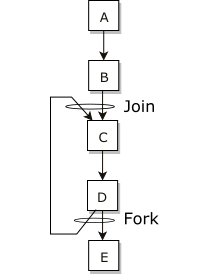
\includegraphics[width=.345\textwidth]{figures/cfg_fork_join_loop_widend}%
\label{fig:fork_join_loop}}
\hfil
\subfloat[Fork-join in an if-else statement.]{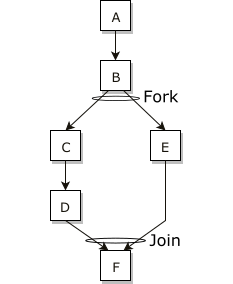
\includegraphics[width=.35\textwidth]{figures/cfg_fork_join_widend}%
\label{fig:fork_join_elif}}
\caption{Fork-join illustration in CFGs.}
\label{fig:fork_join_ill}
\end{figure}

The fork-join model typically branches off (fork) execution at a designated point in the program, and joins (merge) at a subsequent point to resume execution. %In parallel computing, this is a technique often used to spawn multiple processes that execute in parallel, which are at some point joined to sequential execution.
%TODO: if sentence above is added, add illustration of -<==>-
When a value is defined in between the fork and join points, and is forwarded to after the join point, it may be defined in one branch, but not or differently in the other branch/branches. When a bypass is encoded in an instruction, it is statically defined, in the sense that whatever branch is taken the value that is forwarded should always come from the bypass source that is encoded in the instruction. For example, take the following assembly code fragment, whatever path is taken to reach this point, the first source operand is always taken from the \texttt{ALU}, and the second source operand is taken from \texttt{MUL} unit.

\begin{lstlisting}
$join-point:
   add r1, ALU, MUL
\end{lstlisting}

Figure \ref{fig:fork_join_ill} shows two example CFGs with a join point. The following assembly code listings will illustrate how ambiguous bypasses may alter behaviour of the program. After that, a way to resolve such ambiguous behaviour is discussed.

\begin{lstlisting}
$A:
   <@$\vdots$@>
$B:
   nop             || v.addi r9,  r0,  32
   nop             || v.lw   r2,  r9,  0
   nop             || v.lw   r3,  r9,  1
   addi <@\hspace{1px}\textcolor{red!70!black}{r3}\hspace{1px}@>, r0, 16 || v.lw   r4,  r9,  2
   ori  r4, r0, 0  || v.addi r10, r0,  64
$C:
   lw   r6, <@\hspace{1px}\textcolor{red!70!black}{r3}\hspace{1px}@>, 3  || v.add  r12, CP,  r0
   lw   r6, <@\hspace{1px}\textcolor{red!70!black}{r3}\hspace{1px}@>, 2  || v.add  r13, CP,  r0
   lw   r6, <@\hspace{1px}\textcolor{red!70!black}{r3}\hspace{1px}@>, 1  || v.add  r14, CP,  r0
$D:
   nop             || v.mul  r12, r4,  r12
   nop             || v.mul  r13, r3,  r13
   addi r4, r4, 0  || v.add  r9,  CP,  r10
   addi r4, r4, 4  || v.add  r12, r12, r13
   sfne r4, 12     || v.mul  r14, r2,  r14
   bf   $C         || v.add  r14, r14, r12
   addi <@\hspace{1px}\textcolor{red!70!black}{r3}\hspace{1px}@>, r3, 32 || v.sw   r14, r9,  0
$E: <@$\vdots$@>
\end{lstlisting}

The assembly code fragment above for the CFG in Figure \ref{fig:fork_join_loop} shows a 3-by-3 matrix multiplication benchmark. In basic block \texttt{B}, each load operations loads a row from the vector memory. Then, each PE has an entire column stored in the RF. In each loop iteration (\texttt{CD}), one row of values is loaded from CP memory and communicated to the PE elements by basic block \texttt{C}. Subsequently, in block \texttt{D} each element of a row from scalar memory is multiplied with a value from a column. The results of the multiplications are added together, thereby, forming a row of the resulting matrix, which is then stored back to vector memory. 

When using the bypass network to forward a value from one basic block to another basic block, it is required that said value comes from the same bypass source regardless of the predecessor that is executed before it. For the matrix multiplication example, when bypassing the occurrences of \texttt{r3}, the value may be forwarded from \texttt{ALU} when predecessor \texttt{D} is executed, or from bypass source \texttt{WB} when predecessor \texttt{B} is executed. Note that this gives a conflict because \texttt{r3} does not come from the same bypass source in each of the predecessors. Therefore, a fix is required that puts the value in the desired bypass source. 

Considering that there can be any nummer of predecessors, the heuristic developed during this project takes the most frequently executed predecessor block as reference, and fixes all other predecessor to match. In this example, the loop body (\texttt{CD}) is executed more often than the loop header (\texttt{B}). Therefore, block \texttt{B} is modified such that it matches block \texttt{D}. To achieve this it can either swap the last two scalar operations in \texttt{B}. However, a more generic approach would be to insert an instruction at the end of \texttt{B} to put the value in the correct bypass source.

\begin{lstlisting}
$A:
   <@$\vdots$@>
$B:
   sfles r5, r6
   bf    $E
$C:
   <@$\vdots$@>
$D:
   j     $F
   addi  <@\hspace{1px}\textcolor{red!70!black}{r7}\hspace{1px}@>, r7, 5
$E:
   sub   r7, r7, r8
   mul   <@\hspace{1px}\textcolor{red!70!black}{r7}\hspace{1px}@>, r7, 3
$F:
   add   r3, <@\hspace{1px}\textcolor{red!70!black}{r7}\hspace{1px}@>, r5
\end{lstlisting}

The assembly code fragment above corresponds to the CFG in Figure \ref{fig:fork_join_elif}. It illustrates another example where a conflict may occur when forwarding a value over the join point to block \texttt{F}. In predecessor block \texttt{D}, the value in \texttt{r7} can be obtained by forwarding the result produced by the \texttt{ALU}. However, when predecessor block \texttt{E} is executed the value of \texttt{r7} may be forwarded from \texttt{MUL} instead. This conflict can be resolved by the same generic approach, namely, by inserting an operation at the end of either predecessor of \texttt{F} such that the value of \texttt{r7} may be forwarded using an identical bypass source, regardless of which predecessor is executed.
